\pdfoutput=1
\documentclass[pra,twocolumn,showpacs,amsmath,amssymb]{revtex4-2}

\usepackage{graphicx}%Include figure files
\usepackage{dcolumn}%Align table columns on decimal point
\usepackage{bm}% bold math
\usepackage[section]{placeins} %force no floats before section
\usepackage{float}

\setlength{\parskip}{1em}

%\nofiles

\begin{document}

\title{Project 3: The Fermi–Pasta–Ulam–Tsingou Problem}


\author{Christopher McGlinn}
\affiliation{Department of Physics and Astronomy, University
of Delaware, Newark, DE 19716-2570, USA}

\begin{abstract}
We discover and explore the Fermi–Pasta–Ulam–Tsingou problem. A series of masses are attached to each other by a spring with the ends attached to walls. Energy injected into a mode different than the initial mode results in ergodic-like behavior until a super-recurrance occurs where the energy transfers back to the initial. We will show this behavior through analysis of the system. We will also show what happens under different initial conditions and different energy injections.
\end{abstract}

\pacs{05.20.−y}


\maketitle

\section{Introduction} \label{sec:intro}

In 1953, Enrico Fermi, John Pasta, Stanislaw Ulam, and Mary Tsingou conducted a simulation to measure the movement of a vibrating string with a non-linear term. In it, they determined that the system would vary between periodic and ergodic behavior. The experiment measured the energy transfer between different modes, or states of common frequency of oscillation. Here, we will be exploring that experiment.
\par In our system, a series of masses are connected via springs, which, at their ends, connected to walls. The masses vibrate when the masses are displaced from their respective resting location. Since the masses in this experiment will all be equal, the equation of motion can be expressed as such:
\begin{eqnarray}
mx_j = K(x_{j+1} - x_j) + \beta(x_{j+1} - x_j)^3 - \\
K(x_{j} - x_{j - 1}) - \beta(x_{j} - x_{j - 1})^3 \notag
\end{eqnarray}
\par Each mass exhibits periodic behaviour when displaced. This behavior can be viewed as energy in a certain mode. These modes are when each mass moves with the same frequency. Different modes have masses move in different directions to one another. 
\par In this experiment we will show that the movement isn't entirely periodic. The system goes through a cycle of moving between ergodic and periodic behaviour.

\section{Method} \label{sec:method}

First we must define the set of variables for the system. To begin we will introduce a set of dimensionless variables to govern the interactions in the system. We will start off by defining a variable \(m = m_1 + m_2\) and the following sets of equations:
\begin{align}
\bar{x} &= \frac{x}{x_o} \notag \\
\bar{x} &= \frac{x}{x_o} \notag
\end{align}
Then, to normalize the equation, we will define $t_o$ and a new value:
\begin{align}
    t_o = \sqrt{\frac{K}{m}} \notag \\
    \bar{\beta} = x_o^2 \frac{\beta}{K}
\end{align}
Then we drop the bars on the variables for simplicity. This gives us a new, normalized equation for the motion:
\begin{align}
x_j = (x_{j+1} - x_j) + \beta(x_{j+1} - x_j)^3 - \\
(x_{j} - x_{j - 1}) - \beta(x_{j} - x_{j - 1})^3 \notag
\end{align}
We will then evaluate the motion using the Verlet method. However, in order to initialize the method, we will need to define the first two states. For this we will use the Euler-Cromer method:
\begin{align}
x_i = x_{i-1} + v_i \Delta t
\end{align}
For times after the initial two steps, we use the following equation:
\begin{align}
    x_i = 2x_{i-1} - x_{i-2} + a_i \Delta t ^2
\end{align}
This will give us a good approximation of the motion of the system, from which we can calculate the energy in each mode. We can then evaluate the eigenvectors and frequencies of the system using the following equations:
\begin{align}
    e_l(j) = &\sqrt{\frac{2}{N+1}}sin(\frac{\pi l}{N+1}j) \\
    \omega(l) & = | 2sin(\frac{1}{2} \frac{\pi l}{N+1})|
\end{align}
This allows us to find the amplitudes of the nodes via the equation:
\begin{align}
    D_l(t) = \sqrt{\frac{2}{N+1}} \sum_{j=1}^N x_j(t)sin(\frac{\pi l}{N+1}j)
\end{align}
Once we know the amplitudes, we can calculate the total energy in a mode via:
\begin{align}
    E_l(t) = \frac{1}{2}[(\frac{d}{dt} D_l(t))^2 + (\omega_l D_l(t))^2]
\end{align}
Another important quantity we will need is the initial energy per mass, which is similar to the temperature of the system. This is calculated by:
\begin{align}
    \epsilon = \frac{E_l_o(t=0)}{N}
\end{align}
This quantity, when evaluated at 0, will show when the system switches between ergodic and non-ergodic behaviour.

\section{Results} \label{sec:results}

To begin, we will show the system for $\beta = 0, 0.3, 1$.
Let us start by looking at the displacement of the masses. In figure 1 we see the displacement at $t = 0$ and the final time. This shows simple harmonic motion of the masses in the system.
\par However, upon looking at the amplitudes of the system. We can see that $\beta$ plays a factor in how the system evolves. It is subtle, but you can see the amplitude of the second mode fluctuate slightly.
\par In order to understand what is going on, we can further analyze the system by looking at the energy for each $\beta$. In figure 3, the system shows the energy in each mode from the initial and final times. We can see that with an increasing $\beta$, energy is transferred into the other modes. This is the paradox of the system. A mode should not be able to transfer the energy across the modes.


\begin{figure}[t!]
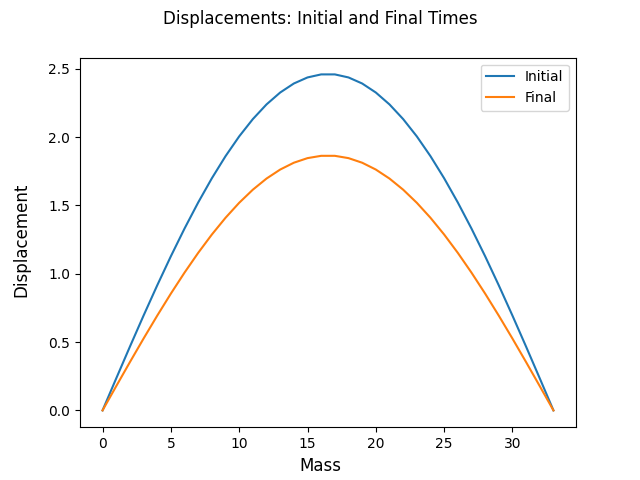
\includegraphics[scale=0.50]{Disp_Beta0.png}
\caption{Displacement of each mass, initial and final times}\label{Poincare1}
\end{figure}

\begin{figure}[t!]
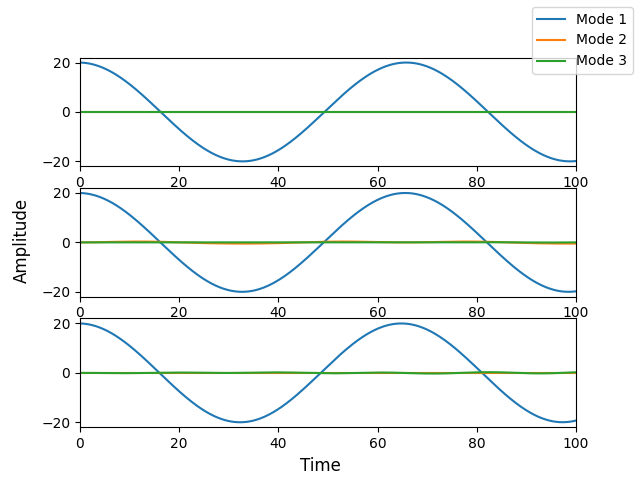
\includegraphics[scale=0.50]{Amp_Betas.png}
\caption{Amplitudes of the first three modes over time for $\beta = 0, 0.3, 1$}\label{Poincare0.5}
\end{figure}

\par While this result appears to be counter to our understanding of physics, it is better explained as we look at the energy of the modes over time. For this, let us look at the most ergodic value, $\beta = 1$. In figure 4, we see that the energy over time does appear to transfer to the other modes. However, after the system is fully evaluated, the energy is transferred back into the initial mode.
\par But what happens when we put the initial energy into another mode? For this, we explored putting the energy into mode 3 and they adjusting the $\beta$ and amplitudes accordingly. In figure 5, we see that this system also transfers the energy into the other modes. However, that energy is transferred back into the initial mode eventually as with the initial system.

\begin{figure}[t!]
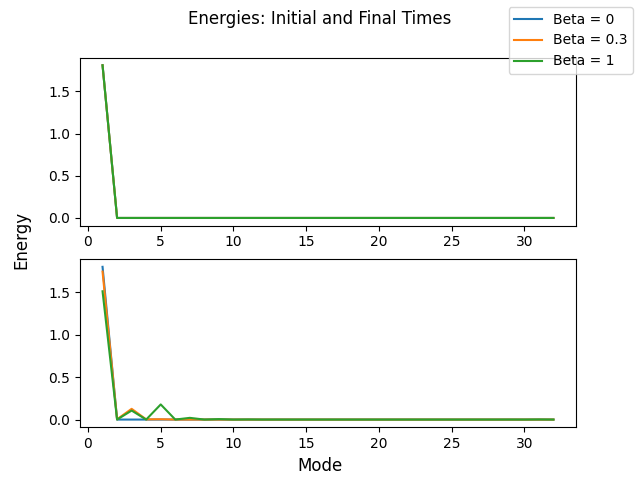
\includegraphics[scale=0.50]{Ene_Betas.png}
\caption{Energy of each mode for $\beta = 0, 0.3, 1$, initial and final times}\label{Poincare9}
\end{figure}

\begin{figure}[t!]
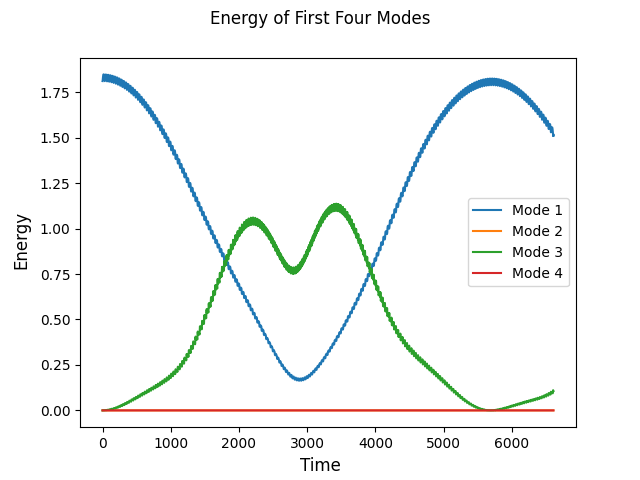
\includegraphics[scale=0.50]{Ene4_Beta1.png}
\caption{Energy of the first four modes for $\beta = 1$}\label{autocorr}
\end{figure}

\par Finally, in figure 6, we see the standard deviation. This shows us the ergodic behaviour of each of the $\beta$ values. This shows the ergodic behavior in the higher $\beta$ values. For $\beta = 0, 0.3$, the deviation remains near 0. However, for $\beta = 1$, the deviation fluctuates.
\par We can look into this further by looking at $\epsilon$. Using a value for the the critical energy per mass, $\epsilon_c$, we can evaluate what the minimum energy per mass of the system such that ergodic behaviour occurs. In figure 7 we see this as a function of $\beta$. The system follows an almost linear decrease.
\par Using a set value for $\beta$, we can then see how this evolves as a function of the number of masses. In figure 8 we can see this further.

\begin{figure}[t!]
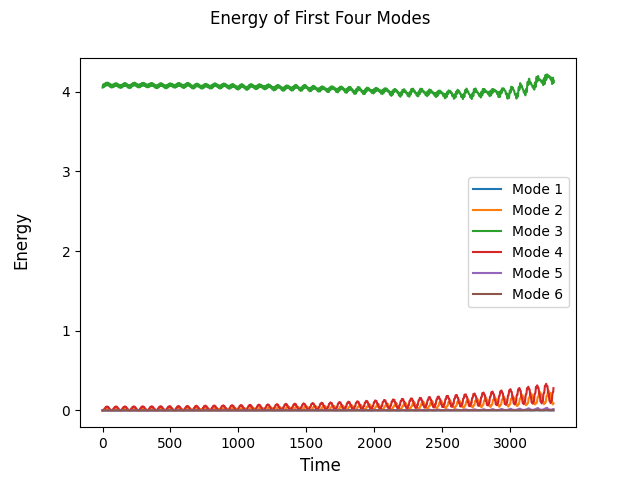
\includegraphics[scale=0.50]{Ene4_Beta03_Mode3.png}
\caption{Energy of the first six modes for $\beta = 0.3$ and the initial energy placed into mode 3}\label{position}
\end{figure}

\begin{figure}[t!]
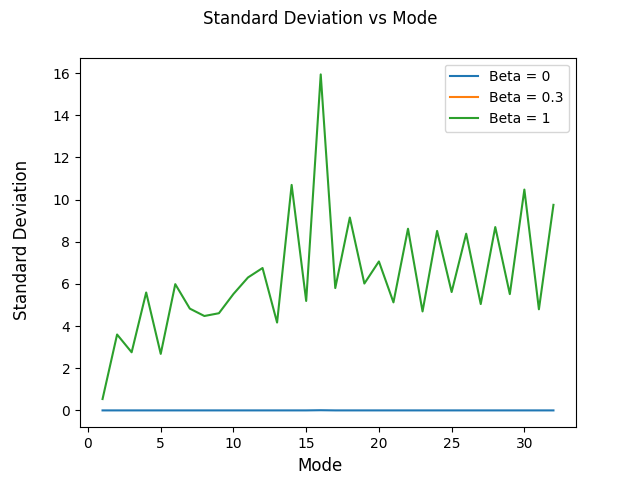
\includegraphics[scale=0.50]{Dev_Betas_16.png}
\caption{Standard deviation for the initial energy in mode 16}\label{position}
\end{figure}

\begin{figure}[t!]
\includegraphics[scale=0.50]{Epsc.png}
\caption{$\epsilon_c$ as a function of $\beta$ in the 32 mass system}\label{position}
\end{figure}

\begin{figure}[t!]
\includegraphics[scale=0.50]{Epsc_N.png}
\caption{$\epsilon_c$ as a function of the number of masses}\label{position}
\end{figure}

\section{Conclusion} \label{sec:conclusion}

In conclusion, we were able to successfully display the Fermi–Pasta–Ulam–Tsingou problem. Looking at the evolution of the energy in each mode over time, we successfully evaluated and displayed what was happening in the system. While a seemingly impossible outcome, it is explained by looking at the system over time. Indeed, the energy is transferred between modes. 
\par However, this is only a temporary transfer. Over time, the energy continues to fluctuate between the modes. The system will eventually transfer its energy back into the initial mode and begin the cycle again.

\begin{thebibliography}{9}
\bibitem{}Nicholas J. Giordano and Hisao Nakanish, \emph{Computational Physics}, (Pearson Prentice Hall, Upper Saddle River NJ,2006).
\end{thebibliography}

\end{document}